%\documentclass[preprint,tightenlines,showpacs,showkeys,floatfix,
%nofootinbib,superscriptaddress,fleqn]{revtex4} 
\documentclass[floatfix,nofootinbib,superscriptaddress,fleqn,preprint]{revtex4} 
%\documentclass[aps,epsfig,tightlines,fleqn]{revtex4}
\usepackage[utf]{kotex}
\usepackage[HWP]{dhucs-interword}
\usepackage[dvips]{color}
\usepackage{graphicx}
\usepackage{bm}
%\usepackage{fancyhdr}
%\usepackage{dcolumn}
\usepackage{defcolor}
\usepackage{amsmath}
\usepackage{amsfonts}
\usepackage{amssymb}
\usepackage{amscd}
\usepackage{amsthm}
\usepackage[utf8]{inputenc}
 \usepackage{setspace}
%\pagestyle{fancy}

\begin{document}

\title{\Large 2022년 1학기 물리학 I: Quiz 6}
\author{김현철\footnote{Office: 5S-436D (면담시간 매주
    화요일-16:00$\sim$20:00)}} 
\email{hchkim@inha.ac.kr}
\affiliation{Hadron Theory Group, Department of Physics,
Inha University, Incheon 22212, Republic of Korea }
\date{Spring semester, 2022}


\vspace{1.cm}
\begin{abstract}
\noindent \textbf{ {\color{red}주의}: \color{blue} 단 한 번의 부정행위도 절대
  용납하지 않습니다. 적발 시, 학점은 F를 받게 됨은 물론이고,
  징계위원회에 회부합니다. One strike out임을 명심하세요.}\\
\\
문제는 다음 쪽부터 나옵니다.  \\ \\
{\bf Date:} 2022년 3월 21일 (월) 15:30-16:15 
\\
{\bf 학번:} \hspace{4cm}
{\bf 이름:} 

\end{abstract}
\maketitle

\noindent {\bf 문제 1 [20pt]}
그림~\ref{fig:1}에서처럼 정지 상태에 있는 세 개의 블록을 가만히
놓았다. 이 세 블록은 $0.500\,\mathrm{m/s^2}$으로 가속한다. 블록 1은
질량이 $M$이고, 블록 2는 $2M$, 블록 3은 $2M$이다. 블록 2와 수평면
사이의 운동마찰계수를 구하여라.
\begin{figure}[ht]
  \centering
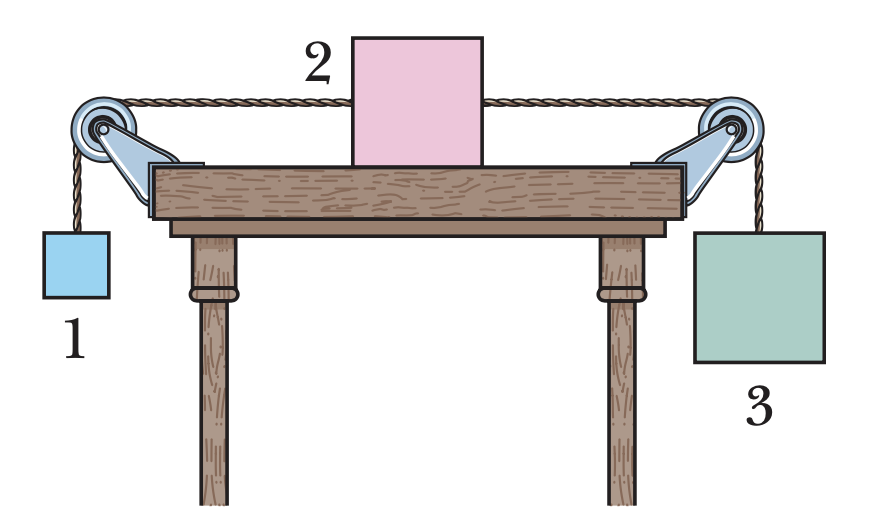
\includegraphics[scale=0.43]{Qfig6-1-20220321.png}  
  \caption{문제 1}
  \label{fig:1}
\end{figure}

\newpage

{\color{gray} [문제 풀이 쪽]}

\newpage 

\noindent {\bf 문제 2 [10pt]} 프라이팬과 달걀 사이의 정지마찰계수는
$\mu_s=0.04$이다. 이 달걀이 프라이팬에서 미끄러지려면 프라이팬은
수평면으로부터 몇 도 기울어져야 하는가?  
\newpage

{\color{gray} [문제 풀이 쪽]}

\newpage 

\noindent {\bf 문제 3 [20pt]}
짐을 실은 승강기의 총 질량이 
$1\,600\,\mathrm{kg}$이다. 초속도 2.00 m/s로 내려오던 승강기가 어느
순간부터 일정한 가속도로 감속하여 5.00 m 더 간 후
정지하였다. 정지하기까지 승강기를 연결한 줄의 장력은 얼마인가? (단,
중력가속도는 $9.80\,\mathrm{m/s^2}$이다.)   
\newpage

{\color{gray} [문제 풀이 쪽]}

\newpage

\noindent {\bf 문제 4 [40pt]} (\textbf{\color{red} 난이도 상})
질량이 각각 $m=16$ kg, $M=88$ kg인 두 블록이 
있다. 그림~\ref{fig:4}처럼 힘 $\vec{F}$를 가해 블록 $m$을 블록 $M$에
맞닿아 있도록 했다. 이 두 블록 사이의 정지마찰계수는
$\mu_s=0.38$이다. 블록 $M$이 놓여있는 수평면과 $M$ 사이에는 쓸림이
없다.  블록 $m$이 블록 $M$에서 미끄러져 내려오지 않도록 하는 데 필요한
최소힘 $\vec{F}$를 구하여라. 
\begin{figure}[ht]
  \centering
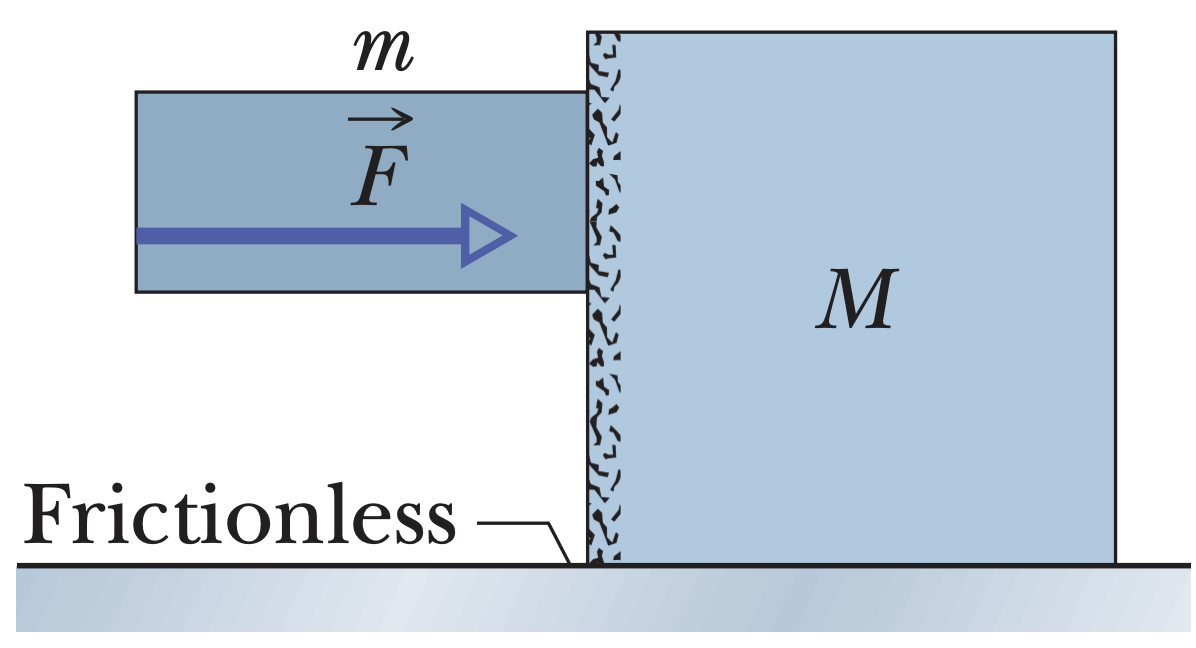
\includegraphics[scale=0.3]{Qfig6-4-20220321.png}  
  \caption{문제 4}
  \label{fig:4}
\end{figure}

\newpage

{\color{gray} [문제 풀이 쪽]}

\newpage
\end{document}